\chapter*{Introduction}
In the last decades, the development of Machine Learning (ML) and Deep Learning (DL) techniques has contaminated every aspect of the scientific world, with interesting results in many different research fields. The biomedical field is no exception to this and a lot of promising applications are taking form, especially as Computer-Aided Detection (CAD) systems which are tools coming in support to physicians during the diagnostic process. Medical doctors and the Healthcare system in general collect a huge amount of data from patients during all the treatment, screening, and analysis activities in many different shapes, from anagraphical data, to blood analysis to clinical images.

In medicine the study of images is ubiquitous and countless diagnostic procedures rely on it, such as X-ray imaging (CAT), nuclear imaging (SPECT, PET), Magnetic resonance, and visual inspection of histological specimens after biopsies. The branch of Artificial Intelligence in the biomedical field that handles image analysis to assist physicians in their clinical decisions goes under the name of Digital Pathology Image Analysis (DPIA).
In this thesis work, I want to focus on some of the beneficial aspects introduced by DPIA in the histological images analysis and some particular issues in the development of DL models able to handle this kind of procedure.

Nowadays the great majority of analysis of histological specimens occurs through visual inspection, carried out by highly qualified experts. Some analysis, as cancer detection, requires the ability to distinguish if a region of tissue is healthy or not with high precision in very wide specimens. This kind of procedure is typically very complex and requires prolonged times of analysis besides substantial economic efforts. Furthermore, the designated personnel for this type of analysis is often limited, leading to delicate issues of priority assignment while scheduling analysis, based on the estimated patient's clinical development. Some sort of support to this analysis procedure is therefore necessary.

The problem of recognizing regions with different features within an image and detect their borders is known in computer vision as segmentation task, and it's quite spread in many different applications, allowing a sort of automatic interpretation of the image. The segmentation problem is usually faced as a supervised task, hence the algorithm in order to be trained properly requires a reasonable quantity of pre-labeled images, from which learn the rules through which distinguish different regions. This means that the development of segmentation algorithms for a specific application, as would be the one with histological images, requires a lot of starting material independently analyzed from the same qualified expert encharged of the visual inspection I mentioned before. A human operator thus is required to manually track the boundaries, for example, between healthy and tumoral regions within a sample of tissue and to label them with their identity, as in Figure \ref{fig:man_seg}. The more the algorithm to train is complex the more starting material is required to adjust the model's parameters and reach the desired efficacy.

\begin{figure}
    \centering
    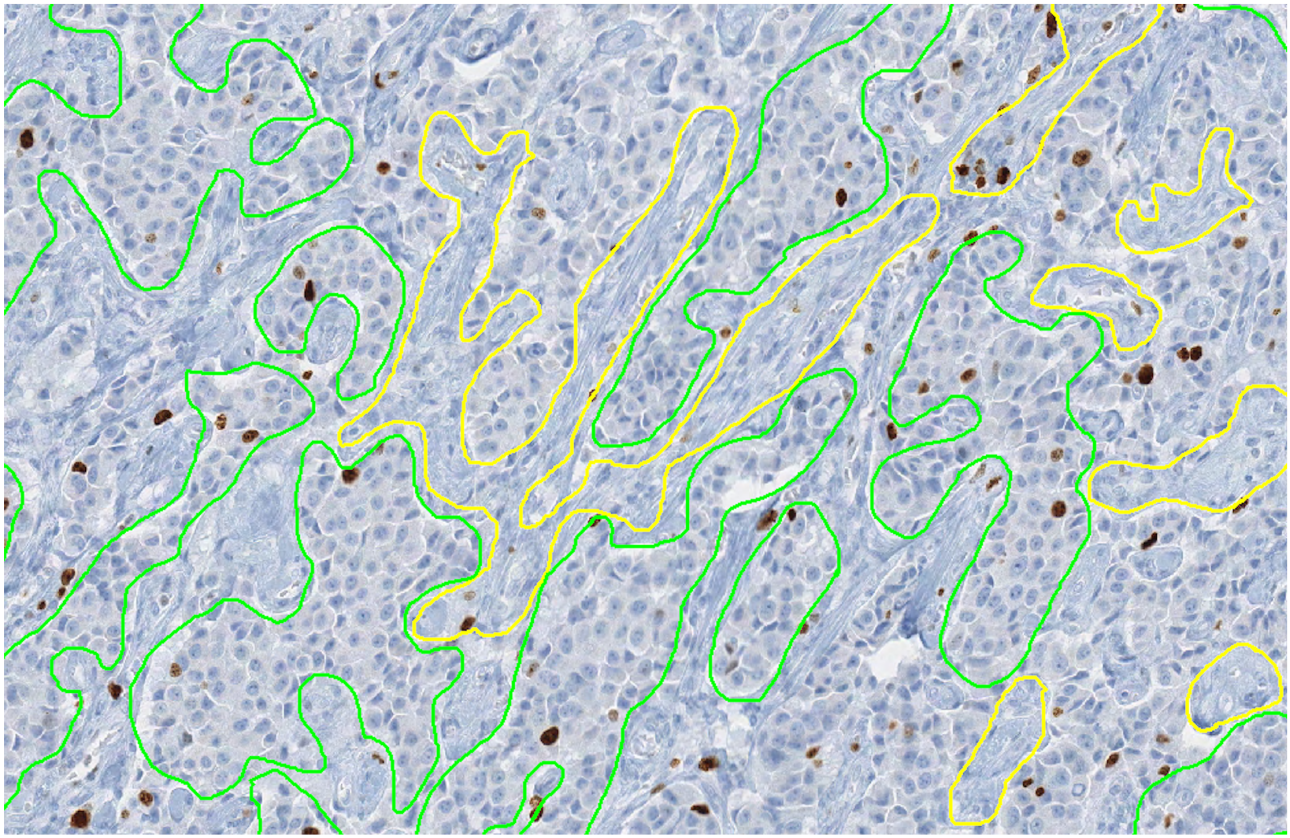
\includegraphics[width = 0.9\textwidth]{images/manual_seg}
    \caption{Interleaving of tumor (green annotation) and non-tumor (yellow annotation) regions \cite{Ki67}.}
    \label{fig:man_seg}
\end{figure}


The latest developed segmentation algorithms are based on DL techniques, hence based on the implementation of intricated Neural Networks (NN) which process the input images end produces the correspondent segmentation. Those models are typically very complex, with millions of parameters to adjust and tune, therefore they need a huge amount of pre-labeled images to learn their segmentation rules. This need for data is exactly the main focus of my thesis work. The shortage of ground truth images is indeed one of the toughest hurdles to overcome during the development of DL-based algorithms. Another important aspect to bear in mind is the quality of the ground truth material. It's impossible for humans to label boundaries of different regions with pixel-perfect precision, while for machines the more precise is the input the more tuned is the resulting algorithm.

There have already been explored different approaches to overcome this problem, and they are mainly based on the generation of synthetic data to be used during the training phase. Some techniques achieve data augmentation manipulating already available images and then generating "new" images, but as we will see later this approach suffers from different issues. The technique that I propose in this work follows a generation from scratch of entire datasets suitable for the training of new algorithms, based on the 3D modelization of a region of human tissue at the cellular level. The sectioning of the virtual histological samples yields the synthetic images with their corresponding ground truth. Using this technique one would be able to collect sufficient material for the training (the entire phase or the preliminary part) of a model, avoiding then the shortage of hand-labeled data.

The 3D modeling of a region of particular human tissue is a very complex task, and it is almost impossible to capture all the physiological richness of a histological system. The models I implemented thus are inevitably schematic in their representation of the target biological structures. I'll show two models: one of pancreatic tissue and another of epidermic tissue, besides all the tools I used and the choices I made during the design phase.


In order to present organically all the steps of my work the thesis is organized in chapters as follows:

\begin{enumerate}
    \item Structure

    \item Of the

    \item Thesys
\end{enumerate}


% \begin{enumerate}
%     \item Description of how histological images are obtained and analysed, and which are the important aspects to take care of.
%     \item Thorough description of the my model for the generation of synthetic images of pancreatic tissue
%     \item Thorough description of the my model for the generation of synthetic images of epidermic tissue
%     \item Introduction to Deep Learning and Segmentation task, and state of the art of DL based segmentation algorithms.
%     \item Future work and improvements
% \end{enumerate}
